\documentclass[10pt]{article}
\usepackage[paperwidth=11.8cm,paperheight=4.5cm,margin=0pt]{geometry}
\usepackage{amsmath,amssymb}
\usepackage{mathptmx}
\renewcommand{\hbar}{\mathchar'26\mkern-9mu h}
\usepackage{tikz}
\pagestyle{empty}
\begin{document}
\special{papersize=11.8cm,4.5cm}
\noindent
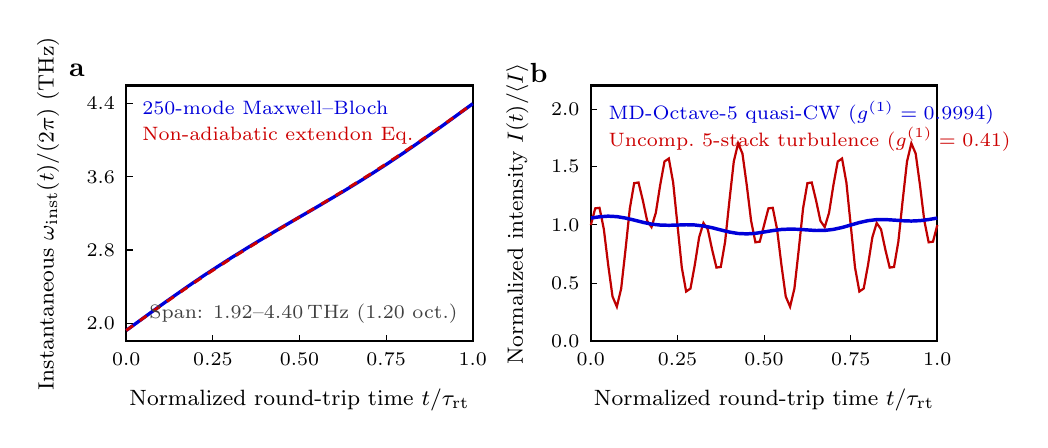
\begin{tikzpicture}[x=1cm,y=1cm,font=\footnotesize]
  % Panel a: Instantaneous frequency chirp across one round trip
  \node[anchor=north west,font=\bfseries\normalsize] at (0.10,4.35) {a};
  \draw[thick] (0.95,0.70) rectangle (5.35,3.95);
  \foreach \v/\y in {2.0/0.93, 2.8/1.86, 3.6/2.79, 4.4/3.72} {
    \draw (0.95,\y) -- (1.03,\y);
    \node[left,font=\scriptsize] at (0.93,\y) {\v};
  }
  \foreach \xval/\xpos in {0.0/0.95, 0.25/2.05, 0.50/3.15, 0.75/4.25, 1.0/5.35} {
    \draw (\xpos,0.70) -- (\xpos,0.78);
    \node[below,font=\scriptsize] at (\xpos,0.68) {\xval};
  }
  \node[below,font=\footnotesize] at (3.15,0.22) {Normalized round-trip time $t/\tau_{\mathrm{rt}}$};
  \node[rotate=90,above,font=\footnotesize] at (0.22,2.32) {Instantaneous $\omega_{\mathrm{inst}}(t)/(2\pi)$ (THz)};

  \draw[blue!85!black,line width=1.2pt] (0.950,0.839) -- (1.060,0.919) -- (1.170,0.999) -- (1.280,1.079) -- (1.390,1.158) -- (1.500,1.236) -- (1.610,1.313) -- (1.720,1.390) -- (1.830,1.465) -- (1.940,1.539) -- (2.050,1.611) -- (2.160,1.682) -- (2.270,1.753) -- (2.380,1.821) -- (2.490,1.889) -- (2.600,1.956) -- (2.710,2.021) -- (2.820,2.086) -- (2.930,2.151) -- (3.040,2.215) -- (3.150,2.279) -- (3.260,2.342) -- (3.370,2.406) -- (3.480,2.471) -- (3.590,2.536) -- (3.700,2.601) -- (3.810,2.668) -- (3.920,2.736) -- (4.030,2.805) -- (4.140,2.875) -- (4.250,2.946) -- (4.360,3.019) -- (4.470,3.092) -- (4.580,3.168) -- (4.690,3.244) -- (4.800,3.321) -- (4.910,3.399) -- (5.020,3.478) -- (5.130,3.558) -- (5.240,3.638) -- (5.350,3.718);
  \draw[red!80!black,dashed,line width=1.05pt] (0.950,0.839) -- (1.060,0.918) -- (1.170,0.997) -- (1.280,1.075) -- (1.390,1.153) -- (1.500,1.230) -- (1.610,1.307) -- (1.720,1.382) -- (1.830,1.457) -- (1.940,1.531) -- (2.050,1.603) -- (2.160,1.674) -- (2.270,1.745) -- (2.380,1.814) -- (2.490,1.882) -- (2.600,1.950) -- (2.710,2.017) -- (2.820,2.083) -- (2.930,2.148) -- (3.040,2.214) -- (3.150,2.279) -- (3.260,2.344) -- (3.370,2.409) -- (3.480,2.474) -- (3.590,2.541) -- (3.700,2.607) -- (3.810,2.675) -- (3.920,2.743) -- (4.030,2.812) -- (4.140,2.883) -- (4.250,2.954) -- (4.360,3.027) -- (4.470,3.100) -- (4.580,3.175) -- (4.690,3.250) -- (4.800,3.327) -- (4.910,3.404) -- (5.020,3.482) -- (5.130,3.560) -- (5.240,3.639) -- (5.350,3.718);

  \node[anchor=north west,font=\scriptsize,blue!85!black] at (1.03,3.88) {250-mode Maxwell--Bloch};
  \node[anchor=north west,font=\scriptsize,red!80!black] at (1.03,3.54) {Non-adiabatic extendon Eq.};
  \node[anchor=south east,font=\scriptsize,black!75] at (5.28,0.80) {Span: $1.92\text{--}4.40\,\mathrm{THz}$ ($1.20$ oct.)};

  % Panel b: Intracavity intensity envelope I(t)
  \node[anchor=north west,font=\bfseries\normalsize] at (5.95,4.35) {b};
  \draw[thick] (6.85,0.70) rectangle (11.25,3.95);
  \foreach \v/\y in {0.0/0.70, 0.5/1.44, 1.0/2.18, 1.5/2.92, 2.0/3.65} {
    \draw (6.85,\y) -- (6.93,\y);
    \node[left,font=\scriptsize] at (6.83,\y) {\v};
  }
  \foreach \xval/\xpos in {0.0/6.85, 0.25/7.95, 0.50/9.05, 0.75/10.15, 1.0/11.25} {
    \draw (\xpos,0.70) -- (\xpos,0.78);
    \node[below,font=\scriptsize] at (\xpos,0.68) {\xval};
  }
  \node[below,font=\footnotesize] at (9.05,0.22) {Normalized round-trip time $t/\tau_{\mathrm{rt}}$};
  \node[rotate=90,above,font=\footnotesize] at (6.18,2.32) {Normalized intensity $I(t)/\langle I\rangle$};

  \draw[red!75!black,line width=0.8pt] (6.850,2.177) -- (6.905,2.389) -- (6.960,2.396) -- (7.015,2.123) -- (7.070,1.671) -- (7.125,1.269) -- (7.180,1.140) -- (7.235,1.371) -- (7.290,1.865) -- (7.345,2.389) -- (7.400,2.709) -- (7.455,2.718) -- (7.510,2.490) -- (7.565,2.231) -- (7.620,2.151) -- (7.675,2.333) -- (7.730,2.683) -- (7.785,2.984) -- (7.840,3.022) -- (7.895,2.718) -- (7.950,2.177) -- (8.005,1.637) -- (8.060,1.333) -- (8.115,1.371) -- (8.170,1.671) -- (8.225,2.022) -- (8.280,2.203) -- (8.335,2.123) -- (8.390,1.865) -- (8.445,1.637) -- (8.500,1.645) -- (8.555,1.966) -- (8.610,2.490) -- (8.665,2.984) -- (8.720,3.215) -- (8.775,3.085) -- (8.830,2.683) -- (8.885,2.231) -- (8.940,1.958) -- (8.995,1.966) -- (9.050,2.177) -- (9.105,2.389) -- (9.160,2.396) -- (9.215,2.123) -- (9.270,1.671) -- (9.325,1.269) -- (9.380,1.140) -- (9.435,1.371) -- (9.490,1.865) -- (9.545,2.389) -- (9.600,2.709) -- (9.655,2.718) -- (9.710,2.490) -- (9.765,2.231) -- (9.820,2.151) -- (9.875,2.333) -- (9.930,2.683) -- (9.985,2.984) -- (10.040,3.022) -- (10.095,2.718) -- (10.150,2.177) -- (10.205,1.637) -- (10.260,1.333) -- (10.315,1.371) -- (10.370,1.671) -- (10.425,2.022) -- (10.480,2.203) -- (10.535,2.123) -- (10.590,1.865) -- (10.645,1.637) -- (10.700,1.645) -- (10.755,1.966) -- (10.810,2.490) -- (10.865,2.984) -- (10.920,3.215) -- (10.975,3.085) -- (11.030,2.683) -- (11.085,2.231) -- (11.140,1.958) -- (11.195,1.966) -- (11.250,2.177);
  \draw[blue!85!black,line width=1.25pt] (6.850,2.266) -- (6.960,2.282) -- (7.070,2.290) -- (7.180,2.284) -- (7.290,2.266) -- (7.400,2.240) -- (7.510,2.212) -- (7.620,2.189) -- (7.730,2.177) -- (7.840,2.174) -- (7.950,2.177) -- (8.060,2.181) -- (8.170,2.178) -- (8.280,2.165) -- (8.390,2.143) -- (8.500,2.115) -- (8.610,2.088) -- (8.720,2.070) -- (8.830,2.065) -- (8.940,2.072) -- (9.050,2.089) -- (9.160,2.107) -- (9.270,2.121) -- (9.380,2.126) -- (9.490,2.123) -- (9.600,2.115) -- (9.710,2.108) -- (9.820,2.109) -- (9.930,2.122) -- (10.040,2.146) -- (10.150,2.177) -- (10.260,2.209) -- (10.370,2.233) -- (10.480,2.246) -- (10.590,2.247) -- (10.700,2.240) -- (10.810,2.232) -- (10.920,2.228) -- (11.030,2.233) -- (11.140,2.247) -- (11.250,2.266);

  \node[anchor=north west,font=\scriptsize,blue!85!black] at (6.95,3.88) {MD-Octave-5 quasi-CW ($g^{(1)}=0.9994$)};
  \node[anchor=north west,font=\scriptsize,red!80!black] at (6.95,3.54) {Uncomp.\ 5-stack turbulence ($g^{(1)}=0.41$)};
\end{tikzpicture}
\end{document}
